%%%%%%%%%%%%%%%%%%%%%%%%%%%%%%%%%%%%%%%%%%%%%%%%%
%%%%%%%%%%%%%%%%%%%%%%%%%%%%%%%%%%%%%%%%%%%%%%%%%

\documentclass[12pt,a4paper]{scrartcl}

%%%%%%%%%%%%%%%%%%%%%%%%%%%%%%%%%%%%%%%%%%%%%%%%%
%%%%%%%%%%%%%%%%%%%%%%%%%%%%%%%%%%%%%%%%%%%%%%%%%

\usepackage[utf8]{inputenc}
\usepackage[english]{babel}
\usepackage[T1]{fontenc}

%%%%%%%%%%%%%%%%%%%%%%%%%%%%%%%%%%%%%%%%%%%%%%%%%
%%%%%%%%%%%%%%%%%%%%%%%%%%%%%%%%%%%%%%%%%%%%%%%%%

%\usepackage{ucs}
\usepackage{amsmath}
\usepackage{amssymb}

%%%%%%%%%%%%%%%%%%%%%%%%%%%%%%%%%%%%%%%%%%%%%%%%%
%%%%%%%%%%%%%%%%%%%%%%%%%%%%%%%%%%%%%%%%%%%%%%%%%

\usepackage{graphicx}
\usepackage{tabularx,colortbl}
\usepackage{capt-of}
\usepackage{booktabs}
\usepackage{hyperref}

%%%%%%%%%%%%%%%%%%%%%%%%%%%%%%%%%%%%%%%%%%%%%%%%%
%%%%%%%%%%%%%%%%%%%%%%%%%%%%%%%%%%%%%%%%%%%%%%%%%

\usepackage{pdflscape}
\usepackage{pdfpages}

%%%%%%%%%%%%%%%%%%%%%%%%%%%%%%%%%%%%%%%%%%%%%%%%%
%%%%%%%%%%%%%%%%%%%%%%%%%%%%%%%%%%%%%%%%%%%%%%%%%

\usepackage[group-separator={,}, group-minimum-digits=3]{siunitx}
\DeclareSIUnit\basepair{bp}

%%%%%%%%%%%%%%%%%%%%%%%%%%%%%%%%%%%%%%%%%%%%%%%%%
%%%%%%%%%%%%%%%%%%%%%%%%%%%%%%%%%%%%%%%%%%%%%%%%%

\usepackage{biocon}
\newtaxon{strain}
\newtaxastyle{WithStrain}{\taxit{\taxonfirst{!genus!.}\taxon{ !epithet!}} str. \#\taxon{!strain!}}

\newanimal{Hd}{genus=Hybsibuis,epithet=dujardini}

%%%%%%%%%%%%%%%%%%%%%%%%%%%%%%%%%%%%%%%%%%%%%%%%%
%%%%%%%%%%%%%%%%%%%%%%%%%%%%%%%%%%%%%%%%%%%%%%%%%

\usepackage{enumitem}
\setlist[enumerate]{itemsep=0mm}

%%%%%%%%%%%%%%%%%%%%%%%%%%%%%%%%%%%%%%%%%%%%%%%%%
%%%%%%%%%%%%%%%%%%%%%%%%%%%%%%%%%%%%%%%%%%%%%%%%%

\usepackage[backend=biber]{biblatex}
\addbibresource{supplement.bib}

%%%%%%%%%%%%%%%%%%%%%%%%%%%%%%%%%%%%%%%%%%%%%%%%%
%%%%%%%%%%%%%%%%%%%%%%%%%%%%%%%%%%%%%%%%%%%%%%%%%

\title{\Large The genome of a tardigrade - \\\large Horizontal gene transfer or bacterial contamination?}
\author{\normalsize Felix Bemm, Clemens Weiß, Jörg Schultz, Frank Förster}
\date{}

%%%%%%%%%%%%%%%%%%%%%%%%%%%%%%%%%%%%%%%%%%%%%%%%%
%%%%%%%%%%%%%%%%%%%%%%%%%%%%%%%%%%%%%%%%%%%%%%%%%

\graphicspath{{./figures/}}
\DeclareGraphicsExtensions{.pdf,.PDF,.png,.PNG,.jpg,.JPG,.jpeg,.JPEG}

%%%%%%%%%%%%%%%%%%%%%%%%%%%%%%%%%%%%%%%%%%%%%%%%%
%%%%%%%%%%%%%%%%%%%%%%%%%%%%%%%%%%%%%%%%%%%%%%%%%

\begin{document}

\maketitle

\pagebreak

\section{Figures}

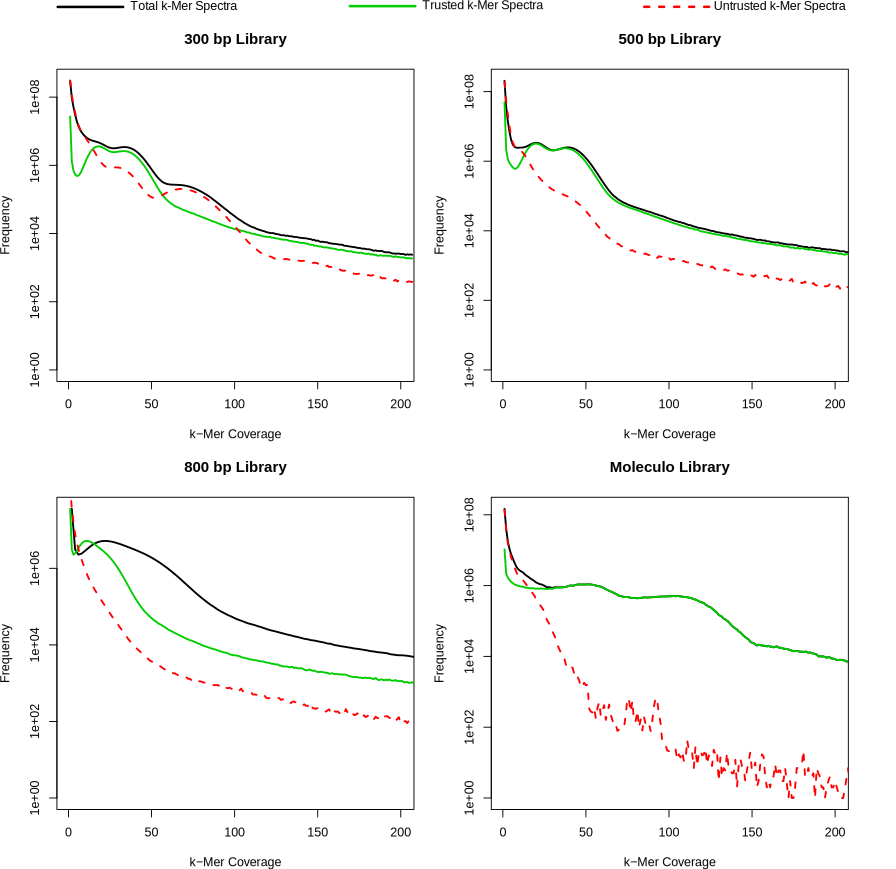
\includegraphics[width=1\textwidth]{supplementary_figure_1}
\captionof{figure}[k-Mer Analysis]{k-Mer Analysis}

\pagebreak

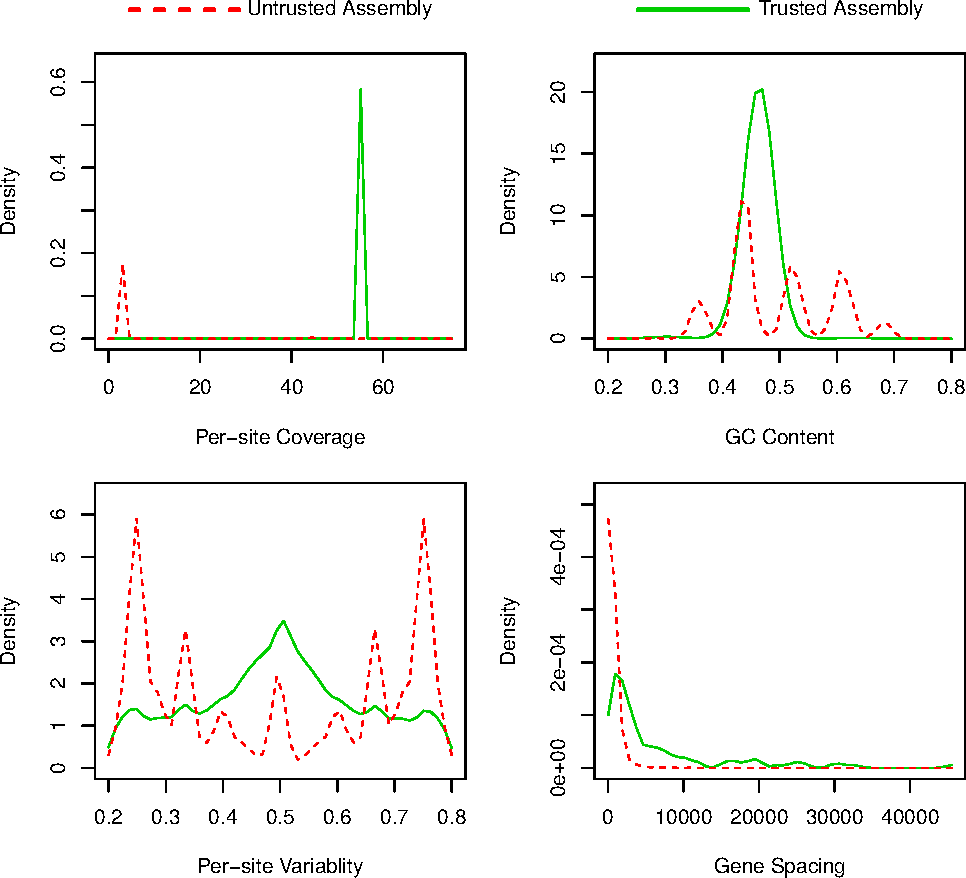
\includegraphics[width=1\textwidth]{supplementary_figure_2}
\captionof{figure}[Assembly Feature Comparisons]{Assembly Feature Comparisons}

\pagebreak

\includegraphics[width=1\textwidth]{supplementary_figure_3}
\captionof{figure}[Unknown Bacterial Genome]{Unknown Bacterial Genome}

\section{Methods}

\subsection*{k-Mer Analysis and Filtering}

Allpaths-LG Jellyfish

\subsection*{Long Read Assembly}

Falcon

\subsection*{Assembly Annotation}

GeneMark-S and GeneMark-ES
CGView -> Visualizatin

\subsection*{Assembly Comparison}

GC Sliding Windows ?
Mapping Coverage ?
Per-site Variability ?
sm-Packages to compare distributions

\printbibliography

\end{document}